\title{Warm-Up for February 28th, 2022}
\author{Dr. Jordan Hanson - Whittier College Dept. of Physics and Astronomy}
\date{\today}
\documentclass[12pt]{article}
\usepackage[a4paper, total={18cm, 27cm}]{geometry}
\usepackage{graphicx}
\usepackage{amsmath}
\usepackage{bm}
\begin{document}
\maketitle

\section{Memory Bank}

\begin{enumerate}
\item Integration by parts in 1D: $\int_a^b u dv = uv|_a^b - \int v du$
\item Integration by parts in 3D: $\int_{\mathcal{V}} (\nabla \cdot \mathbf{E}) V d\tau = \oint_{\mathcal{S}} V \mathbf{E} \cdot d\mathbf{A} - \int_{\mathcal{V}} \mathbf{E} \cdot (\nabla V) d\tau$
\item Work required to assemble a continuous charge distribution: $W = \frac{1}{2} \int \rho V(\mathbf{r}) d\tau$
\end{enumerate}

\begin{figure}[ht]
\centering
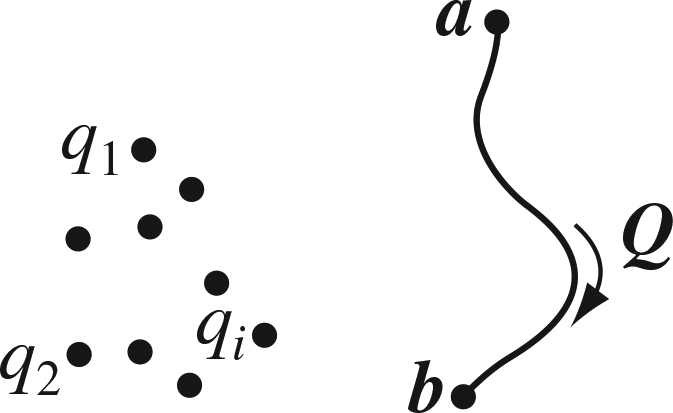
\includegraphics[width=0.2\textwidth]{figures/2_39.jpg}
\caption{\label{fig:charges} By bringing a new charge toward a charge distribution, we are performing work: $W = Q\Delta V = Q (V(\mathbf{r}) - V(\infty))$.}
\end{figure}

\section{Product Rule}

Using the product rule, show that

\begin{equation}
\int_0^{\infty} x e^{-x} dx = 1
\end{equation}

\vspace{1cm}

\section{Work and Energy}

Using items 2 and 3 in the memory bank and $\rho = \epsilon_0 \nabla \cdot \mathbf{E}$, show that the work to assemble a charge distribution is

\begin{equation}
W = \frac{\epsilon_0}{2} \left[ \oint V \mathbf{E} \cdot d\mathbf{a} - \int \mathbf{E} \cdot (\nabla V) d\tau \right]
\end{equation}

Substitute $\mathbf{E} = -\nabla V$ to find how $W \propto E^2$.

\end{document}